\documentclass[a4paper,12pt]{article}

% --- Slovenské prostredie ---
\usepackage[slovak]{babel}
\usepackage[utf8]{inputenc}
\usepackage[T1]{fontenc}
\usepackage{csquotes}
\usepackage[backend=biber,style=numeric,language=english]{biblatex}

% --- Grafika, tabuľky, formátovanie ---
\usepackage{graphicx}
\usepackage{amsmath}
\usepackage{booktabs}
\usepackage{caption}
\usepackage{geometry}
\geometry{margin=2.5cm}
\usepackage{float}
\usepackage{subcaption} 

% --- Citácie ---
\addbibresource{references.bib}

% --- Odseky ---
\setlength{\parskip}{0.5em}
\setlength{\parindent}{0pt}

\begin{document}

% ===============================
% TITULNÁ STRANA
% ===============================
\begin{titlepage}
    \centering
    {\Large \textbf{Technická univerzita v Košiciach}}\\[0.3em]
    {\large Fakulta elektrotechniky a informatiky}\\[0.3em]
    {\large Katedra kybernetiky a umelej inteligencie}\\[2cm]
    
    \vspace*{\fill}
    {\huge \textbf{Extrahovanie kľúčových slov z dokumentov}}\\[1cm]
    {\Large Semestrálne zadanie}\\[0.3em]
    {\large Manažment znalostí}\\
    {\large Zimný semester 2025/2026}\\
    \vspace*{\fill}
    
    \begin{flushright}
        {\large Bc. Boris Daňko}\\
        {\large Bc. Roland Palgut}\\
        {\large Bc. Marek Puškáš}\\[1cm]
        {\large Košice, \today}
    \end{flushright}
\end{titlepage}


% ===============================
% OBSAH
% ===============================
\tableofcontents
\newpage
\setcounter{tocdepth}{2}

% ===============================
% TEXT PRÁCE
% ===============================

\section{Popis problému}

V súčasnosti dochádza k neustálemu rastu objemu digitálnych dát vo forme textových dokumentov, vedeckých článkov, správ, e-mailov či príspevkov na sociálnych sieťach. Táto expanzia textových dát vyvoláva potrebu efektívnych metód na ich automatizované spracovanie, analýzu a porozumenie obsahu. Jednou z kľúčových úloh v oblasti spracovania prirodzeného jazyka (Natural Language Processing - NLP) a dolovania textu (Text Mining) je extrakcia kľúčových slov (Keyword Extraction - KE). 

Cieľom extrakcie kľúčových slov je identifikovať tie termíny, ktoré najlepšie vystihujú obsah a tému daného dokumentu. Kľúčové slová majú zásadný význam pri úlohách, ako sú sumarizácia textu, klasifikácia dokumentov, vyhľadávanie informácií či automatické značkovanie obsahu \cite{rose2010automatic}. Automatizovaná extrakcia kľúčových slov zároveň znižuje časovú náročnosť manuálneho anotovania a umožňuje spracovávať rozsiahle textové korpusy bez zásahu človeka.

Podľa štúdie \cite{rose2010automatic} sú hlavné výzvy v tejto oblasti spojené s presnosťou a spoľahlivosťou extrakcie. Tradičné štatistické prístupy (napr. Log-Likelihood Test - LLT) často vykazujú závislosť od referenčných korpusov, čím sa znižuje ich robustnosť. Problémom býva aj nedostatočné filtrovanie neplnovýznamových slov, ako sú predložky či spojky, ktoré dosahujú vysokú frekvenciu, no nenesú významovú hodnotu.

Ďalšou významnou výzvou je rozpoznávanie viacslovných termov (multi-word expressions) a doménovo špecifických kľúčových pojmov, ktoré sa nemusia vyskytovať v štandardných lexikálnych databázach. Moderné prístupy preto čoraz viac využívajú sémantické modely, ktoré umožňujú zachytiť významové súvislosti medzi slovami, nielen ich frekvenciu výskytu.

Problém extrakcie kľúčových slov je úzko spätý aj s inými úlohami spracovania textu, ako je sumarizácia dokumentov či automatizované odpovedanie na otázky (Question Answering - QA). Moderné extraktory kľúčových slov a sumarizačné systémy využívajú modely typu BERT alebo KeyBERT \cite{grootendorst2020keybert}, ktoré umožňujú systémom lepšie pochopiť kontext používateľského dopytu a prispôsobiť mu výslednú sumarizáciu či extrakciu informácií.

Celkovo možno povedať, že problém extrakcie kľúčových slov spočíva v potrebe vytvoriť metódu, ktorá bude presná, doménovo prispôsobiteľná a nezávislá od manuálneho zásahu človeka. Takáto metóda by mala zohľadniť nielen frekvenčné charakteristiky slov, ale aj ich sémantické a štylistické väzby v rámci textu.

\section{Popis existujúcich metód}

Extrakcia kľúčových slov sa historicky vyvíjala od jednoduchých štatistických prístupov až po moderné modely založené na hlbokých neurónových sieťach. V tejto časti sú predstavené najpoužívanejšie prístupy, ktoré sa vyskytujú v literatúre a prezentáciách k text miningu.

\subsection{Tradičné modely pre vyhľadávanie informácií}

V oblasti vyhľadávania informácií (Information Retrieval - IR) existujú tri základné klasické modely \cite{manning2008introduction}:

\begin{enumerate}
    \item \textbf{Boolovský model} - predstavuje najjednoduchší prístup, v ktorom sú dokumenty a dopyty reprezentované ako množiny termov. Vyhľadávanie je založené na logických operátoroch AND, OR, NOT. Tento model je efektívny, ale neumožňuje určiť mieru relevancie dokumentu.
    
    \item \textbf{Vektorový model} - dokumenty aj dopyty sú reprezentované ako vektory termov v n-dimenzionálnom priestore. Miera podobnosti sa počíta pomocou kosínusovej podobnosti, pričom váhovanie termov je najčastejšie realizované pomocou metódy TF-IDF.
    
    \item \textbf{Pravdepodobnostný model} - odhaduje pravdepodobnosť, že používateľ považuje dokument za relevantný pre svoj dopyt. Tento prístup predstavuje základ pre moderné re-ranking algoritmy v systémoch vyhľadávania informácií.
\end{enumerate}

\subsection{Štatistické metódy - LLT a TF-IDF}

Tradičné korpusovo orientované metódy, ako napríklad \textbf{Dunningov Log-Likelihood Test (LLT)}, patria medzi najstaršie prístupy ku kľúčovosti slov \cite{dunning1993accurate}. LLT hodnotí štatistickú významnosť rozdielov vo frekvencii slov medzi cieľovým a referenčným korpusom. Slová s výrazne vyššou frekvenciou v cieľovom korpuse sú považované za kľúčové. Nevýhodou LLT je jeho závislosť od kvality referenčného korpusu a neschopnosť pracovať s významovou redundanciou.

Naopak, metóda \textbf{Term Frequency-Inverse Document Frequency (TF-IDF)} \cite{salton1988term} je jednou z najpoužívanejších techník v NLP. Hodnotí dôležitosť termu na základe jeho relatívnej frekvencie v rámci dokumentu a zriedkavosti v celom korpuse. TF-IDF umožňuje jednoduché, ale účinné určenie relevantných termov bez potreby referenčného korpusu. Využíva sa nielen v extrakcii kľúčových slov, ale aj vo vyhľadávačoch, odporúčacích systémoch či textovej klasifikácii.

Štúdia \cite{rose2011tfidf} navrhuje vylepšenú verziu TF-IDF, ktorá zohľadňuje distribúciu slov naprieč dokumentmi a filtruje gramatické slová s nízkou informačnou hodnotou. Táto metóda využíva vnútorné štatistiky korpusu a eliminuje potrebu externých dát, čím sa zvyšuje jej prenositeľnosť a univerzálnosť.

\subsection{Latentné sémantické a vektorové modely}

Moderné NLP techniky rozširujú pôvodné frekvenčné metódy o sémantické chápanie textu. \textbf{Latentné sémantické indexovanie (LSI)} využíva singulárnu dekompozíciu matíc (SVD) na zistenie skrytých významových vzťahov medzi slovami a dokumentmi \cite{deerwester1990indexing}. Umožňuje redukciu dimenzie a potláča problémy synonymie a polysémie, ktoré sú typické pre prirodzený jazyk.

Ďalším krokom boli modely založené na distribučných reprezentáciách, ako \textbf{Word2Vec}, \textbf{GloVe} a neskôr \textbf{BERT}, ktoré umožňujú zachytiť význam slov na základe ich kontextu. Takéto modely sú základom moderných extrakčných nástrojov, ako napríklad \textbf{KeyBERT}, ktorý využíva vektorové reprezentácie a kosínusovú podobnosť na určenie najrelevantnejších kľúčových slov v texte \cite{grootendorst2020keybert}.

\subsection{Transformátorové a hybridné metódy}

Najnovšie prístupy v oblasti extrakcie kľúčových slov využívajú \textbf{transformátorové architektúry} (napr. BERT, T5, PEGASUS), ktoré umožňujú pochopiť kontext textu na hlbšej úrovni \cite{devlin2019bert, lewis2020bart, zhang2020pegasus}. Tieto modely dokážu kombinovať informácie o sémantike, gramatike aj pragmatike jazyka a sú vhodné pre úlohy, kde je dôležité pochopiť zámer a význam celého dokumentu.

V oblasti sumarizácie a odpovedania na otázky (Question Answering) sa objavujú metódy, ktoré využívajú extrahované kľúčové slová na navádzanie modelu počas generovania sumarizovaného textu \cite{grootendorst2020keybert}. Takéto prístupy spájajú extrakciu a generáciu a predstavujú prechod k hybridným systémom schopným integrovať viaceré NLP techniky.

\subsection{Zhrnutie}

Klasické metódy (LLT, TF-IDF) sú výpočtovo jednoduché a interpretovateľné, no často ignorujú významové súvislosti. Na druhej strane, moderné vektorové a transformátorové prístupy umožňujú modelom pochopiť kontext a význam slov, ale vyžadujú veľké množstvo dát a výpočtových zdrojov. V praxi sa preto často používajú \textbf{hybridné riešenia}, ktoré kombinujú štatistické váhovanie s vektorovou reprezentáciou textu, čím sa dosahuje kompromis medzi efektivitou a presnosťou extrakcie.

\section{Návrh metódy a výber testovacích dát}

Cieľom navrhovanej metódy je umožniť flexibilnú a modulárnu extrakciu kľúčových slov z textových dokumentov rôznych typov, ako sú PDF alebo TXT súbory. Metóda kombinuje tri prístupy: TF-IDF, YAKE a KeyBERT, pričom každý z nich poskytuje odlišný spôsob hodnotenia významu termov v dokumente.  

\begin{itemize}
    \item \textbf{TF-IDF} vyhodnocuje relatívnu dôležitosť termov na základe ich frekvencie v dokumente a zriedkavosti naprieč korpusom.
    \item \textbf{YAKE} je nezávislý, korpusovo orientovaný algoritmus založený na štatistike n-gramov a váh slov.
    \item \textbf{KeyBERT} využíva moderné transformátorové modely (BERT), ktoré zachytávajú kontext a význam slov vo vete, vrátane možnosti použitia Maximal Marginal Relevance (MMR) pre diverzifikované kľúčové slová.
\end{itemize}

Všetky metódy umožňujú upravovať parametre, ako sú počet extrahovaných kľúčových slov, rozsah n-gramov alebo diverzita v KeyBERT, čo umožňuje testovanie na rôznych typoch textov a dopytoch.

Pre testovanie metódy boli použité dva zdroje dát:  

\begin{enumerate}
    \item \textbf{Vlastné nahrané dokumenty} - používateľ môže nahrať ľubovoľný súbor vo formáte TXT alebo PDF a overiť spracovanie reálnych textových dát.
    \item \textbf{Vzorky zo zložky DATA/} - pripravené textové súbory s rôznou dĺžkou a obsahom, slúžiace na porovnanie výkonu a presnosti jednotlivých metód.
\end{enumerate}

Pred spracovaním textu sa vykonáva predspracovanie, ktoré odstraňuje nadbytočné medzery, čísla a špeciálne znaky, čím sa zvyšuje kvalita extrahovaných kľúčových slov.

\section{Experimentovanie a vyhodnotenie}

Po implementácii metódy boli vykonané experimenty s cieľom porovnať kvalitu a relevantnosť kľúčových slov generovaných rôznymi prístupmi. Pre každý dokument sa extrahovali kľúčové slová pomocou TF-IDF, YAKE a KeyBERT a výsledky sa vizualizovali prostredníctvom barových grafov a wordcloudov.

Hlavné parametre testované počas experimentov boli:  
\begin{itemize}
    \item \textbf{Počet kľúčových slov} (top\_n)
    \item \textbf{Rozsah n-gramov}
    \item \textbf{Diverzita v KeyBERT} pri použití MMR
\end{itemize}

% \subsection{TF-IDF}

\begin{figure}[htbp]
    \centering
    \begin{subfigure}[b]{0.45\textwidth}
        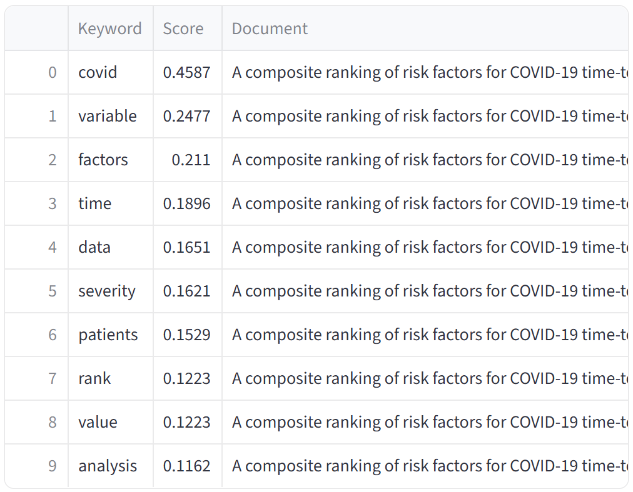
\includegraphics[width=\textwidth]{../images/tfidf_table.png}
        \caption{Tabuľka kľúčových slov TF-IDF}
        \label{fig:tfidf_table}
    \end{subfigure}
    \hfill
    \begin{subfigure}[b]{0.45\textwidth}
        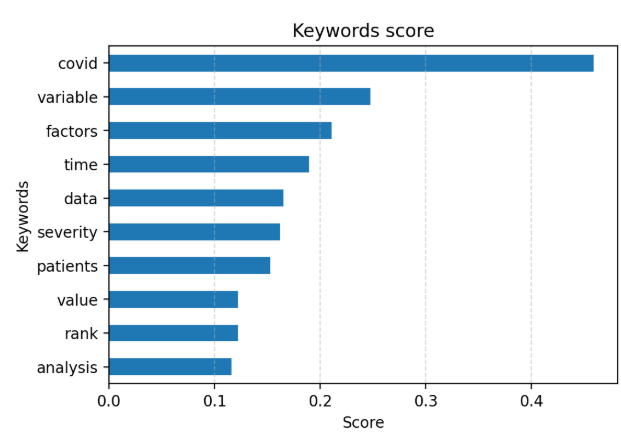
\includegraphics[width=\textwidth]{../images/tfidf_barh.png}
        \caption{Barh graf TF-IDF}
        \label{fig:tfidf_barh}
    \end{subfigure}

    \vspace{0.5cm}

    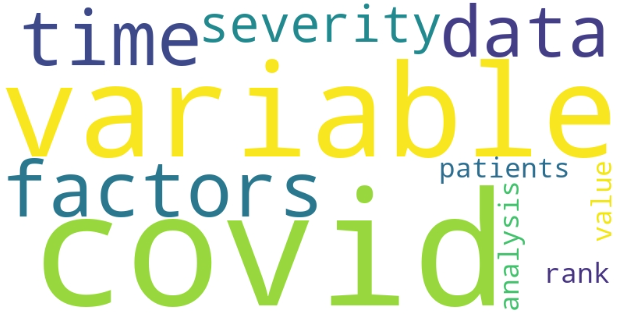
\includegraphics[width=0.6\textwidth]{../images/tfidf_wordcloud.png}
    \caption{Výsledok extrakcie kľúčových slov metódou TF-IDF}
    \label{fig:tfidf}
\end{figure}


% \subsection{YAKE}

\begin{figure}[htbp]
    \centering
    \begin{subfigure}{0.45\textwidth}
        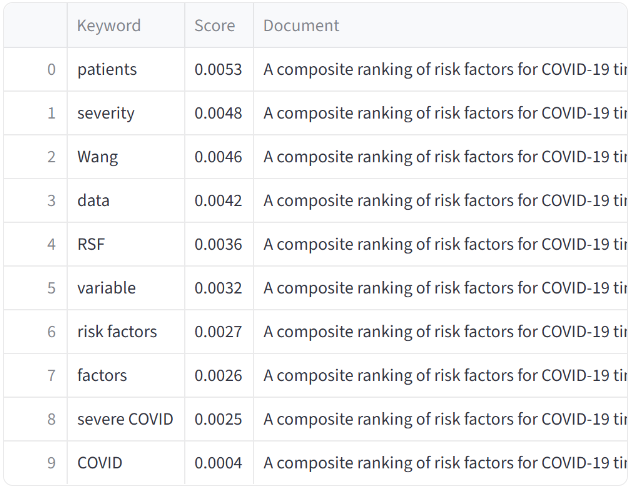
\includegraphics[width=\textwidth]{../images/yake_table.png}
        \caption{Tabuľka kľúčových slov YAKE}
    \end{subfigure}
    \hfill
    \begin{subfigure}{0.45\textwidth}
        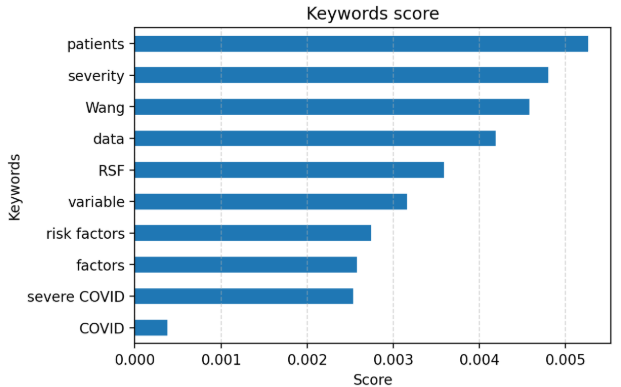
\includegraphics[width=\textwidth]{../images/yake_barh.png}
        \caption{Barh graf YAKE}
    \end{subfigure}

    \vspace{0.5cm}

    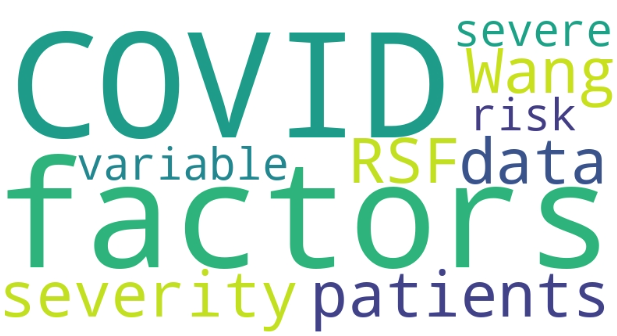
\includegraphics[width=0.6\textwidth]{../images/yake_wordcloud.png}
    \caption{Výsledok extrakcie kľúčových slov metódou YAKE}
    \label{fig:yake}
\end{figure}

% \subsection{KeyBERT}

\begin{figure}[htbp]
    \centering
    \begin{subfigure}{0.45\textwidth}
        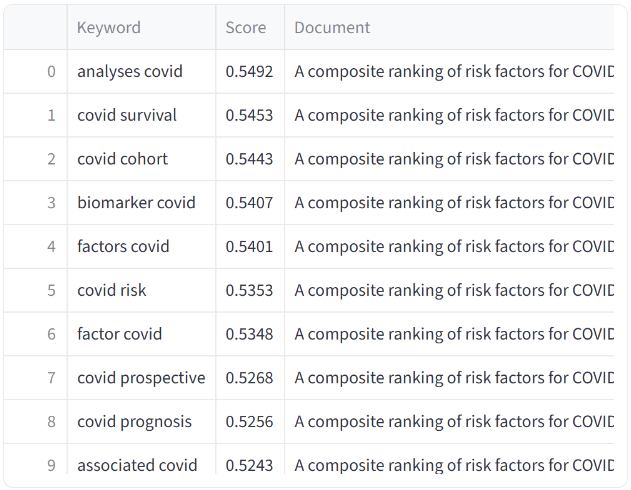
\includegraphics[width=\textwidth]{../images/keybert_table.png}
        \caption{Tabuľka kľúčových slov KeyBERT}
    \end{subfigure}
    \hfill
    \begin{subfigure}{0.45\textwidth}
        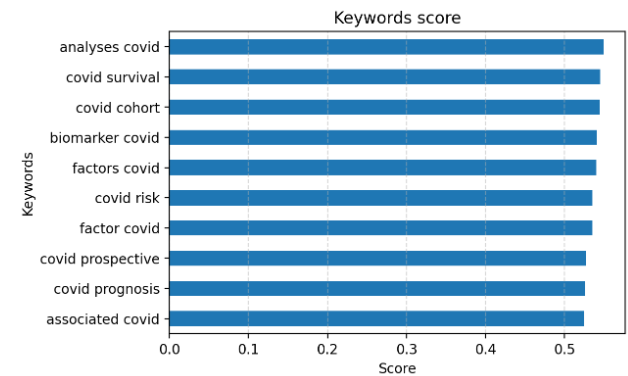
\includegraphics[width=\textwidth]{../images/keybert_barh.png}
        \caption{Barh graf KeyBERT}
    \end{subfigure}

    \vspace{0.5cm}

    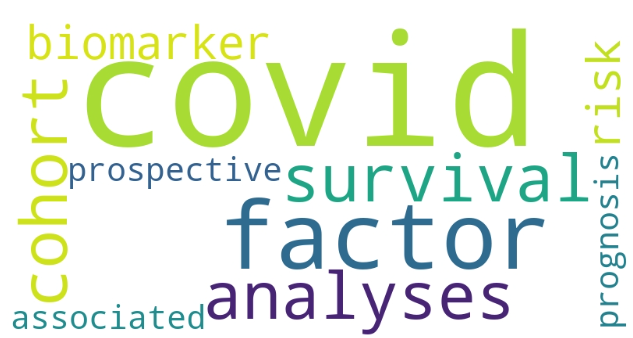
\includegraphics[width=0.6\textwidth]{../images/keybert_wordcloud.png}
    \caption{Výsledok extrakcie kľúčových slov metódou KeyBERT}
    \label{fig:keybert}
\end{figure}

\subsection{Zhrnutie experimentov}

\begin{itemize}
    \item TF-IDF je rýchly a účinný pre kratšie dokumenty s jasne definovanými termami.
    \item YAKE eliminuje bežné stopwords a irelevantné výrazy.
    \item KeyBERT poskytuje najlepší kontextový opis, hlavne pri viacslovných termoch; MMR zvyšuje diverzitu výsledkov.
\end{itemize}

\noindent
Kombinácia týchto metód poskytuje robustný nástroj na extrakciu kľúčových slov a umožňuje prispôsobiť parametre podľa typu a dĺžky dokumentu.

% ===============================
% BIBLIOGRAFIA
% ===============================
\clearpage
\printbibliography[heading=bibnumbered]


\end{document}
